\documentclass{jsarticle}

\renewcommand{\labelenumii}{\theenumii}
\renewcommand{\theenumii}{\theenumi.\arabic{enumii}.}

% Font
\usepackage[platex]{otf}
%\renewcommand{\textbf}[1]{{\bfseries\sffamily#1}}
% \usepackage{times}
%\usepackage[deluxe,expert]{otf}
%\renewcommand{\textbf}[1]{{\bfseries\sffamily#1}}

%\renewcommand{\textbf}{} % TODO: enable blod font for japanese.

% Graphics
\usepackage[dvipdfmx,hiresbb]{graphicx}
\usepackage{array, booktabs}
\usepackage{subcaption}

% Algorithm
\usepackage{algorithm}
\usepackage{algorithmic}
\captionsetup[algorithm]{labelformat=empty}

% index
\usepackage{makeidx}
\makeindex

% Hypertext
\usepackage[dvipdfmx]{hyperref}

% Utility
\usepackage{comment}

% Style
%\usepackage{ijcai15}

\title{マルチコアマシンにおける\\
並列A*探索の探索オーバーヘッドの定性的な解析と\\
アルゴリズムの再評価}
\author{陣内 佑 \\
東京大学教養学部学際科学科\\
\\
指導教員 福永 Alex}

\begin{document}

\maketitle

\begin{abstract}
% Why study A*?
グラフ探索問題のうち最も重要なものの一つとして、辺にコストのついた有向グラフ、初期状態、ゴール状態を入力とし、初期状態からゴール状態までの経路のうちコストが最小である経路を出力する問題がある。この問題を解く為の代表的なアルゴリズムのフレームワークとしてA*探索がある。このA*探索を並列化する手法は数多く提案されている。

% Why study HDA*?
HDA*は特に分散メモリ環境において効率的な並列A*探索である。
HDA*は各スレッドに対してオープンリスト・クローズドリストをローカルに置き、スレッド間で非同期的に仕事を分配する。HDA*は探索済のノードの全てをクローズドリストに保存する為、Transposition Driven Schedulingなどの探索済ノードの一部しか保存しないアプローチと比較して余剰な展開ノードが少ない。しかしHDA*はPBNFと比較して余剰な展開ノードが生じるという先行研究が存在する。PBNFは共有メモリ環境においてstate-of-the-artとされる手法である。PBNFがHDA*よりも優れる理由としては余剰な展開ノードの数が小さいことが指摘されている。しかしながら、先行研究によるHDA*とPBNFの性能比較実験は複数問題点がある。

% What am I going to do?
本研究はまず、HDA*の余剰な展開ノードを定性的に分析し、その原因を3つに分類する。また、問題サイズが十分に大きい場合、それらのオーバーヘッドが無視出来る大きさであることを理論的・実験的に示す。
次に、先行研究におけるHDA*とPBNFの性能比較実験の問題点を指摘し、その上でより詳細な性能比較実験を行う。その実験結果として、 (1) 両アルゴリズムで展開ノード数は大きく変わらないこと、 (2) 逐次実行で10秒程度以上の問題ではHDA*の方がパフォーマンスに優れることを示す。
\end{abstract}

\newpage
\tableofcontents
\newpage

\section{序論}

\subsection{研究の背景}
% Why should we study this?
グラフは情報科学に通底する問題ドメインであり、グラフを解き明かす探索アルゴリズムは分野の基本骨子をなしている。人工知能の分野においても探索は基盤となるアルゴリズムの一つであり、高速で効率的な探索アルゴリズムを研究することは人工知能於いては情報科学全体に意義のある研究である。さて、近年単一プロセッサの高速化は電力の限界を迎え、並列化による高速化へとパラダイムが移った。ハードウェアは今後も各CPUの計算速度の発展よりも並列化による高速化が進むだろうと予測されている。%要注釈 
故に今後ハードウェアの高速化の恩恵を引き出す為にはこの並列システムを利用したアルゴリズムを開発する必要がある。然るに探索アルゴリズムも単一プロセッサによる探索だけではなく、マルチコア・分散システムにおいてもそれぞれ効率的なアルゴリズムを研究しなければならない。


\subsection{関連研究}

グラフを探索するアルゴリズムのうち最も重要なものの一つとしてA*(エースター)アルゴリズムがある\cite{Hart1968}。このA*アルゴリズムを並列化する手法は数多く提案されている。
\newline

% Parallel A*の説明
Kumarらはオープンリスト, クローズドリストをスレッド間で共有して並列に探索を行うParallel A*を提案し、性能評価を行った\cite{Kumar1988parallel}。この手法はオープンリスト, クローズドリストのデータ構造を保つ為に相互排他ロックを必要とする。ノードが展開される度にオープンリストに、生成される度にクローズドリストにロックを獲得してアクセスする必要がある。その為Parallel A*は同期オーバーヘッドが非常に大きいという問題がある。\ref{sec:analysis2}章で見るように、このシンプルな手法は逐次A*よりも遅くなってしまう。
\newline

% HDA*の説明

同期オーバーヘッドを解決する手法としてKishimotoらはHash Distributed A*(HDA*)を提案した\cite{Kishimoto2013}。HDA*は各スレッドにローカルにオープンリストとクローズドリストを持つ。グラフのノードはHash関数によって均等かつ無作為に分割し各スレッドに割り当てられる。各スレッドは自分に割り当てられたノードのみを展開し、他スレッドに割り当てられたノードを生成した場合はそのスレッドにノードを非同期的に送信する。各スレッドのオープンリスト、クローズドリストは他のスレッドからアクセスされないので、相互排他ロックを必要としない。その為HDA*は同期オーバーヘッドが殆どない。HDA*は同期オーバーヘッドが殆どなく、スレッド間でノードの送信以外に大きな情報の通信を必要としないので、特に分散メモリ環境で有効な手法である。また、アルゴリズムの論理が非常にシンプルであるという利点もある。HDA*は逐次A*と比較してHash関数による分配が必要なだけであり、各スレッドの処理は逐次A*と殆ど同様である。並列アルゴリズムはデバッグが難しい為、シンプルであるということは非常に価値がある。HDA*の問題点としても、展開ノード数が大きくなることが指摘されている。HDA*において展開ノード数が増加する原因はまだ調べられていない。また、Kishimotoらの性能評価は殆ど分散メモリ環境におけるものであり、共有メモリ環境における実験は殆ど行われていない。また、それらも共有メモリ環境に最適化された実装を用いたものではない。その為、HDA*のマルチコアマシンにおける性能評価は不十分であると言える。
\newline

% PBNF TODO: 複雑さの上手い説明方法は?
Burnsらは共有メモリ環境における並列化手法としてParallel Best-NBlock-First (PBNF)を提案した\cite{Burns2010}。PBNFは状態空間を複数のNBlockに分割する。それぞれのNBlockはオープンリストとクローズドリストを持つ。それぞれのスレッドは最も有望なノードを持つNBlockを占有し、探索を行う。自分の占有しているNBlockよりも有望なノードを持つNBlockが空いていれば、今探索していたNBlockを解放し、新しいNBlockを占有して探索を始める。あまりに頻繁なNBlockの切り替えが生じるのを防ぐために最小展開ノード数が設定される。これはチューニングの必要なパラメータである。NBlockはスレッドに占有されるので、オープンリスト・クローズドリストに相互排他ロックをかける必要がない。必要なロックは空いているNBlockを保存するheapのみである。その為PBNFは同期オーバーヘッドが小さい。PBNFは分散メモリ環境では有効ではないが、現在共有メモリ環境で最もパフォーマンスの良いstate-of-the-artの手法であるとされている。PBNFの問題点として、その複雑さが挙げられる。すなわち、PBNFのパフォーマンスを引き出す為には空間をNBlockに分割する方法・粒度と最小展開ノード数をドメインに対して最適化をする必要がある。
\newline

% HDA* vs PBNF比較実験の問題点
BurnsらはマルチコアマシンでHDA*を含めた様々な並列アルゴリズムの性能比較を行い、その中でPBNFとHDA*を有望な(高速な)アルゴリズムとした。その上でPBNFはHDA*より速いと結論をした。その理由としては、PBNFはHDA*よりも探索ノード数が小さいという結果があったことを指摘した。しかしながら、Burnsらの比較実験には複数問題点がある。KishimotoらのHDA*の実装がZobrist Hash\cite{Zobrist1970}を用いていたのに対してBurnsらはNaiveなHash関数を用いている。Hash関数によってHDA*の性能は大きく異なると考えられるが、その違いは検証されていない。また、オープンリストをheapで実装しているが、これはBurnsらがベンチマーク問題として扱っている15 Puzzle、4 way Grid-pathfindingにおいて最適な実装ではない\cite{Burns2012implementing}。もう一つ重要な問題点として、ベンチマーク問題のサイズが小さいということが挙げられる。並列アルゴリズムは初期化に時間がかかる為、ある程度問題サイズが大きいものでないと実質的な高速化効率を正確に測ることが出来ない。Burnsらの用いた問題集はA*探索で10秒未満のものが多く、それらが十分な大きさであるかは検証の必要がある。
\newline

これらの理由から、HDA*とPBNFはより詳細な性能評価が必要であると考えられる。また、HDA*のHash関数による挙動の違いも重要な問題である。また、両アルゴリズムのオープンリストの実装がそれぞれどのような影響を与えるかも調査する必要がある。

\subsection{研究の目的}

本研究の目的は2つある。

\begin{enumerate}
\item HDA*の探索ノード数の増加の原因を分析する。
\newline

HDA*におけるノードの探索順をA*と比較をすることで探索ノード数の増加の原因を分析する。また、Hash関数が探索順に与える影響を比較する。HDA*のノードの展開速度を遅くした場合の比較も行う。
\newline

\item マルチコア環境において、HDA*とSafePBNFの性能評価を行う。
\newline

まず、HDA*のhash関数を変えた際の性能を比較する。次にHDA*とSafePBNFのオープンリストの実装をvectorとheapにした場合の性能を比較する。それらの結果を踏まえ、最適なHDA*とSafePBNFの実装をもって性能の比較を行う。

\end{enumerate}


\subsection{本論文の構成}

本論文は以下の通りに構成される。
\ref{sec:define}章でA*探索の詳細とA*探索の並列化手法について述べる。\ref{sec:domain}章は本研究で扱うベンチマーク問題の問題ドメインについて解説する。\ref{sec:analysis1}章はHDA*の探索ノード数の増加を解析する。\ref{sec:analysis2}章ではHDA*とSafePBNFのチューンアップを行ったのち、性能の比較評価を行う。\ref{sec:conclusion}章は本研究で行った実験・解析から得られる知見をまとめる。

\section{A*探索とその並列化}
\label{sec:define}
\subsection{A*探索}
\index{A*, A*探索}
\index{逐次A*}

A*探索アルゴリズム(A*, A*探索)はヒューリスティック関数によって、展開された探索空間の中で最も有望であるノードを推定し、そのノードを優先して探索するアルゴリズムである\cite{Hart1968}。ヒューリスティック関数を利用しないブラインド探索と比較して高速に最適解を見つけられることが多い。A*探索は以下のようなアルゴリズムである。

\begin{enumerate}
	\item 初期状態をオープンリストに加える。
	\item オープンリストにあるノードの中でゴール状態までの見積りが最小であるノードを展開する。
	\begin{enumerate}
		\item 展開したノードをオープンリストから取り除き、クローズドリストにその状態を加える。
		\item 展開した状態がゴール状態かどうかを調べる。ゴール状態である場合は解を出力して終了する。
		\item 目標状態でない場合、展開した状態から1つの行為で遷移可能な状態のうち、クローズドリストにないすべての状態をオープンリストに加える。
	\end{enumerate}
	\item オープンリストが空になった場合は解なしとして終了する。
\end{enumerate}

オープンリスト\index{オープンリスト}は未探索のノード、クローズドリスト\index{クローズドリスト}は探索済のノードが保存されるデータ構造である。あるノード$n$からゴール状態までの見積り$f(n)$は$f(n) = g(n) + h(n)$で計算される。$g(n)$は初期状態からノード$n$までの経路にかかったコストである。$h(n)$は状態からゴール状態までの距離を推定する\textbf{ヒューリスティック関数}\index{ヒューリスティック、ヒューリスティック関数}である。ヒューリスティック関数が\textbf{admissible}\index{admissible}であるならば、A*探索の解の最適性が保証される。ヒューリスティック関数がadmissibleであるとは、ゴール状態までの推定コストを過小に見積もることがないということである。



以降の議論では、並列化したアルゴリズムと区別する為に\textbf{逐次A*}と呼ぶ。


\subsection{A*探索の並列化にかかるオーバーヘッド}

並列探索は、理想的にはスレッドの数だけ高速化する。しかしながら、一般に並列探索は並列に伴うオーバーヘッドが生じる。並列化のオーバーヘッドは以下の3つに分類される。

\begin{enumerate}
\item 探索オーバーヘッド\index{探索オーバーヘッド}
\newline

一般に並列探索は逐次A*よりも多くのノードの展開を必要とする。並列化に伴い余剰に展開したノードの割合を探索オーバーヘッドと呼ぶ。本研究では、探索オーバーヘッドは以下の式によって推定する。
\newline
\begin{equation}
	SO := \frac{並列実行によって展開したノード数}{逐次実行によって展開したノード数}
\end{equation}


$SO$は理想的には1になるが、多くの場合1よりも大きくなる。
\newline

\item 同期オーバーヘッド\index{同期オーバーヘッド}
\newline

同期オーバーヘッドは、他スレッドの処理を待つ為にアイドル状態で待たなければならない場合に生じる。データ構造の一部は同時に複数のスレッドがアクセスすることが出来ない。そのようなデータ構造をスレッド間で共有する場合は相互排他ロック(ロック)\index{相互排他ロック}を必要とする。相互排他ロックは、ロックを獲得したスレッド以外のスレッドによるアクセスを禁止する制御機構である。あるスレッドが他スレッドによって獲得された相互排他ロックが解放されるまで待つ場合、同期オーバーヘッドとなる。相互排他ロックを必要としないか、ロックの解放を待たずに他の処理に移る場合を非同期通信\index{非同期通信}と呼ぶ。
\newline

\item 通信オーバーヘッド\index{通信オーバーヘッド}
\newline

通信オーバーヘッドはスレッド間の通信にかかる遅延である。スレッド間の通信は仕事の分配や情報の共有の為に行われる。

\end{enumerate}

これらのオーバーヘッドはトレードオフの関係にある。理論的にこれらを最小にすることは非常に困難である為、多くの場合は実験的に最適な実装にチューニングが行われる。

並列化にかかるオーバーヘッドの計測の為には\textbf{高速化効率(efficiency)}\index{高速化効率}\index{Efficiency}という指標が用いられる。Efficiencyは以下のように定義される。
\newline

\begin{equation}
	\mbox{Efficiency} := \frac{逐次実行による実行時間}{並列実行による実行時間 \times スレッドの数} % TODO: fの字体を修正
\end{equation}

Efficiencyは理想的には1になるが、上述のオーバーヘッドがかかる為に多くの場合1未満である。Efficiencyが1の場合を\textbf{Perfect linear speedup}\index{Perfect linear speedup}と呼ぶ。Efficiencyが1を越える場合を\textbf{Superlinear speedup}\index{Superlinear speedup}と呼ぶ。

本研究では探索オーバーヘッドと高速化効率を主な指標として用いる。

\subsection{Parallel A*}
\index{Parallel A*}
最もシンプルなA*の並列化手法はKumarらの提案した\textbf{Parallel A*}である\cite{Kumar1988parallel}。Parallel A*は各スレッドでA*探索を行う。スレッド間でオープンリスト, クローズドリストを共有することで並列に探索をすることが出来る。この手法はオープンリスト, クローズドリストのデータ構造を保つ為に相互排他ロックを必要とする。各スレッドはノードを展開する度にオープンリストに、ノードを生成する度にクローズドリストにロックを獲得してアクセスする必要がある。その為Parallel A*は同期オーバーヘッドが非常に大きいという問題がある。\ref{sec:analysis2}章で見るように、このシンプルな手法は逐次A*よりも遅くなってしまう。以降、Parallel A*は特にこの手法を指す。


\subsection{Parallel Retracting A* (PRA*)}
\index{Parallel Retracting A*, PRA*}
% まずPRA*とTDSの説明を行い、比較したHDA*の利点の説明
% HDA*はParallel Retracting A* (PRA*)とTransposition-table driven work scheduling (TDS)のアイディアを発展させた手法である。
% PRA*の説明
Parallel Retracting A* (PRA*)は各スレッドにローカルにオープンリストとクローズドリストを持つ\cite{evett1995massively}。グラフのノードはHash関数によって均等かつ無作為に分割し各スレッドに割り当てられる。各スレッドは自分に割り当てられたノードのみを探索し、他スレッドに割り当てられたノードを生成した場合はそのスレッドにノードを同期的に送信する。Hash関数が均等かつ無作為な分割であれば、仕事の分配は均等であり、全てのスレッドが効率的に仕事をすることが出来る。また、クローズドリストをローカルに置くことが出来るので、分散メモリ環境においても効率的に重複の確認が可能である。ノードの送信時、送信側のスレッドは受信側のスレッドが受信の態勢に入るのを待ち、受信側スレッドは受信に成功したら送信側スレッドにそれを報告する。送信側スレッドはその報告を受け取るまで待機しなければならない。この為PRA*は同期オーバーヘッドが大きいという問題がある。
\newline

MahapatraとDuttはPRA*で提案されたHash関数による仕事の分配をより深く研究した\cite{mahapatra1997scalable}。
彼らはまず、PRA*で提案されたHash関数による分配をSEL\_SEQ\_A*に適応したアルゴリズムをGlobal Hashing of Nodes (GOHA)と定義して実装をした。SEL\_SEQ\_A*はA*探索の変化形であり、ノードの展開時に$f$値の大きいノードの生成を後周しにする手法である。その上で、彼らはGOHAの変化形として2つの手法を提案した。一つはGOHAにQuality Equalizingのメカニズムを適応したGlobal Hashing of Nodes and Quality Equalizing (GOHA\&QE)である。この手法は異なるメカニズムで重複の確認と仕事の分配を行う。一度オーナーに重複がないことが確認されたノードは、どのプロセスで展開しても問題ない。GOHA\&QEは仕事を効率的に分配する為に、重複の確認後に更に各プロセスの仕事の質に応じて仕事の再分配を行う。GOHA及びGOHA\&QEで使われるHash関数はグローバルであり、ノードはあるプロセッサからどのプロセッサにも送信される可能性がある。一般に、並列コンピュータアーキテクチャにおいて、プロセッサ同士の通信コストはペア毎に異なる。よって、このようなHash関数は最適ではない可能性がある。Local Hashing of Nodes and Quality Equalizinig (LOHA\&QE)は探索空間を複数のグループに分割し、隣り合うグループが隣り合うプロセッサに割り当てる手法である。MahapatraとDuttはTravelling Salesperson Problemにおいてこれらの手法が単純なPRA*よりもパフォーマンスに優れることを示した。この手法はコンピュータのアーキテクチャに依存し、かつLOHAは問題ドメインに対して複数の前提を必要とするという問題点がある。

\subsection{Transposition-table driven work scheduling (TDS)}
\index{Transposition-table driven work scheduling, TDS}
% TODO: TDSの説明を詳しく
Transposition-table driven work scheduling (TDS)は分散メモリ環境におけるIDA*の並列アルゴリズムである\cite{romein1999transposition}。
TDSはPRA*同様にHash関数によって仕事を分配する。Transposition-tableはノードの重複を調べる為に使われるキャッシュであり、プロセッサの数だけ分割されている。Transposition-tableによる重複の確認により、TDSは逐次のIDA*よりも余剰に展開するノード数が非常に小さい。TDSは分散メモリ環境で、特に15 PuzzleやRubik's cubeなどの問題で効率的であると示されている。また、TDSの基礎となるアイディアは二人零和ゲームにも応用されている。


% HDA*の定義
\subsection{Hash Distributed A* (HDA*)}
\index{Hash Distributed A*, HDA*}
HDA*はPRA*で提案されたHashによる仕事の分配メカニズムに基づく手法である。
各スレッドはローカルにオープンリストとクローズドリストを持つ。グラフのノードはHash関数によって均等かつ無作為に分割し各スレッドに割り当てられる。各スレッドは自分に割り当てられたノードのみを探索し、他スレッドに割り当てられたノードを生成した場合はそのスレッドにノードを非同期的に送信する。

% 改めてPRA*, TDSとの比較
PRA*は同期的な通信によってノードの送受信を行うのに対して、HDA*は非同期的に通信を行い、他のスレッドの処理を待たない。その為、HDA*は同期オーバーヘッドが殆どない。TDSは探索深度を更新するイテレーション毎に多くのノードが再展開される。HDA*はA*探索の並列化であるので、このような再展開はない。TDSはIDA*の並列化手法であるのに対し、HDA*はA*の並列化手法である。HDA*はTDSのようにノードの再展開をする必要がなく、展開ノード数が小さいというメリットがある。HDA*は計算機の環境に依存せず、分散メモリ環境・共有メモリ環境の両方で効率的である。また、問題ドメインに依存せずに実装が出来るシンプルな手法である。
\newline

HDA*の処理は以下の通りである。
HDA*はまず、ルートプロセスで初期状態を展開する。その後、それぞれのスレッド$P$は最適解を発見するまで以下のループを繰り返す。

\begin{enumerate}
	\item $P$は自分のメッセージキューに新しいノードが入っているかを確認する。もし入っていたら、それぞれのノードを$P$のクローズドリストと照合し、オープンリストに入れるべきかを確認する。
	\item メッセージキューが空なら、$P$のオープンリストから最も優先度の高いノードを展開し、新しいノードを生成する。生成されたノード$s$に対してそれぞれハッシュキー$K(s)$を計算する。ノード$s$は$K(s)$を担当するプロセッサのメッセージキューに送信される。この送信は非同期的で、ロックを必要としない。$P$は送信先からの返信を待たずに次の計算に移る。
\end{enumerate}

% Hash関数
HDA*のHash関数はHDA*の性能に非常に重要である。Hash関数に求められる要件は以下である。

\begin{enumerate}
	\item 全てのスレッドに対してなるべく均等される。
	\item 状態空間に対してなるべく不偏かつ均等な分配である。
	\item Hash値を高速に求めることが出来る。
\end{enumerate}

以上の要件から、多くのドメインにおいて\textbf{Zobrist Hash}\index{Zobrist Hash}が使われる\cite{Zobrist1970}。ノード$s$の状態が整数列$\mathbf{x}$で表現されるとする。状態の$i$番目の整数の取りうる値は$l_{i}$通りあるとする。ノードの状態を$\mathbf{x} = (x_{0}, x_{1}, …, x_{n})$と置く。この時$x_{i}$は$0 \leq x_{i} < l_{i}$である。$R_{i}$を$l_{i}$個の値を持つテーブルとする。$R_{i}$は予めランダムに生成される。ここでZobrist Function $Z(s)$は以下のように定義される。
\newline
\begin{equation}
	Z(s) := R_{0}[x_{0}]\; xor\; R_{1}[x_{1}]\; xor\; …\; xor\; R_{n}[x_{n}]%
\end{equation}

$R_{i}$はランダムに生成される為、$Z(s)$は均等な確率で定義域の全ての値が出ると期待される。また、状態の全情報を利用して生成される為、局所的な状態の変化に対しても不偏な分配を行うことが出来る。$xor$によって計算する為、親ノードからの差分のみを計算してHash値を求めることが出来る。加えて、XOR命令は非常に速い計算である。よってZobrist Hashは高速に求めることが出来る。

% アルゴリズムの停止方法


% TODO: Parallel Structured Duplicate Detectionの説明を入れる
\subsection{Parallel Structured Duplicate Detection}
\index{Parallel Structured Duplicate Detection, PSDD}
Parallel Structured Duplicate Detection (PSDD)はPRA*とは異なる並列化のフレームワークである\cite{zhou2007parallel}。
PSDDはロックを取得する回数とスレッド間でノードを通信する回数を減らすことを目的として設計された。PSDDはstructured duplicate detection (SDD)で提案されたアイディアに基づく手法である\cite{zhou2004structured}。SDDはabstract functionによって複数のノードを1つのグループにまとめ、これをnblockと呼ぶ。それぞれのnblockはオープンリストとクローズドリストを持つ。nblockで展開されたノードの子が分配されうるnblockの集合を、そのnblockのduplicate detection scopeと呼ぶ。各スレッドはnblockの探索する時に、このduplicate detection scopeを排他的に専有する。よって、PSDDはノードの展開時にロックを必要としない。ノードの展開は最も多い処理の一つであるので、これにロックを必要としないことは大きな利点である。加えて、生成されたノードはスレッドの専有するduplicate detection scope内のnblockに配置される為、他のスレッドと通信をする必要がない。

\subsection{Parallel Best-NBlock First (PBNF, SafePBNF)}
\index{Parallel Best-NBlock First, PBNF}
\index{SafePBNF}
Parallel Best-NBlock First (PBNF)はPSDDのフレームワークを最良優先探索に適応したアルゴリズムである。PBNFは状態空間を複数のNBlock\index{NBlock}に分割し、各スレッドがNBlockを交換しながら探索する\cite{Burns2010}。それぞれのNBlockはオープンリストとクローズドリストを持つ。それぞれのスレッドは最も有望なノードを持つNBlockを占有し、探索を行う。また、占有したNBlockに隣接するNBlockをスレッドのinterference scopeに加える。他のスレッドのinterference scopeに加わったNBlockを探索することは出来ない。同一のNBlockは複数のinterference scopeに入ることが出来る。自分の占有しているNBlockよりも有望なノードを持つNBlockが空いていれば、今探索していたNBlockとinterference scopeを解放し、新しいNBlockを占有して探索を始める。このとき、あまりに頻繁なNBlockの切り替えが生じるのを防ぐために、NBlockを切り替える前に探索する最小のノード数が設定される。これはチューニングの必要なパラメータである。NBlockはスレッドに占有されるので、オープンリスト・クローズドリストに相互排他ロックをかける必要がない。必要なロックは空いているNBlockを保存するheapのみである。
\newline

% Livelock
PBNFはLivelockが起こる可能性がある。Livelockは、複数のスレッドが同じ資源を解放する処理を実行しているにも拘らず、どちらのスレッドも資源が獲得出来ない状況である。この時、アルゴリズムは有限時間内に終了しないことになる。あるNBlockが複数のスレッドのinterference scopeに入っている場合、どのスレッドもそのNBlockを探索することが出来ない状態になりうる。Burnsらはこの問題を解決したSafePBNFを提案し、SafePBNFにおいてLivelockが発生しないことを証明した。SafePBNFはLivelockを防ぐ為にNBlockに対してhotというフラグを定義する。あるNBlockが複数のスレッドのinterference scopeに入っている場合、このNBlockをhotとする。hotなNBlockを探索する要求があった場合、そのNBlockをinterference scopeに含むスレッドは現在探索しているNBlockを解放する。これによって、Livelockを防ぐことが出来る。
\newline

% Why SafePBNF, not PBNF?
Livelockの可能性のあるアルゴリズムは完全ではない。アルゴリズムが完全であるとは、健全性と停止性を満たすことである。健全性とはアルゴリズムの結果が正しいことであり、停止性とはどのような入力に対しても有限時間内に結果を出力して停止することである。PBNFはLivelockが生じる可能性があるので、停止性を満たさない。PBNFは完全ではないのに対して、SafePBNFは完全である。本研究で扱うA*, Parallel A*, HDA*は全て完全なアルゴリズムである。よって、同じ完全なアルゴリズムであるSafePBNFを比較の対象とする。

\begin{algorithm}                      
\caption{PBNF search framework}         
\label{alg:pbnf}                          
\begin{algorithmic}                  
\WHILE {there is an nblock with open nodes}
	\STATE lock; $b \leftarrow$ best free nblock; unlock
	\WHILE {$b$ is no worse than the best free nblock or we've done fewer than $m$ expansions}
		\STATE $n \leftarrow$ best open node in $b$
		\IF {$f(n) \leq f(incumbent)$}
			\STATE prune all open nodes in $b$
		\ELSIF { $n$ is a goal }
			\STATE $incumbent \leftarrow n$
		\ELSE 
			\STATE for each child $c$ of $n$
			\STATE insert $c$ in the open list of the appropriate nblock
		\ENDIF
\ENDWHILE
\ENDWHILE
\end{algorithmic}
\end{algorithm}



\section{問題ドメイン}
\label{sec:domain}

\subsection{Sliding-tile Puzzle (15 Puzzle, 24 Puzzle)}
\index{Sliding-tile Puzzle, 15 Puzzle, 24 Puzzle}

\begin{figure}
	\centering
	\includegraphics[width=0.3\columnwidth]{others/15puzzle.png}
	\caption{Sliding-tile Puzzle}
	\label{fig:15puzzle}
\end{figure}% 
% What is slinding tile puzzle? % TODO: 過去形?現在形?
図\ref{fig:15puzzle}のように、四角い枠にタイルが敷き詰められている。枠には一ヶ所タイルのない場所があり、そこに縦と横からタイルをスライドすることが出来る。\textbf{Sliding-tile Puzzle}は、タイルのスライドによって初期状態から特定のゴール状態まで動かす経路を求める問題である。15 Puzzleの状態空間の大きさはおよそ$10^{13}$状態、24 Puzzleの状態空間はおよそ$10^{25}$状態である。 本研究では15 Puzzleのヒューリスティック関数は\textbf{マンハッタン距離}\index{マンハッタン距離}を用いた。マンハッタン距離ヒューリスティックは、各タイルのゴール状態での位置までのマンハッタン距離の総和で求められる。タイルは同時に2つ動かすことは出来ない。また、あるタイルがゴール位置に動かす為には少なくともマンハッタン距離の回数だけ動かす必要がある。よって、マンハッタン距離ヒューリスティックはadmissibleなヒューリスティック関数である。
\newline

% Why 15 Puzzle as the main benchmark?
15 Puzzleはノードの展開が非常に高速なドメインである。ノードの展開が速いドメインは並列化によって高速化することが困難である。なぜならば、展開が高速である分、同期オーバーヘッドや通信オーバーヘッドによる遅延の影響が大きくなるからである。15 Puzzleドメインにおいて高速化が可能であれば、多くのドメインにおいても同様に高速化が可能であると考えられる。この理由から、15 Puzzleは並列探索のベンチマーク問題として広く使われている。本研究でも主に15 Puzzleをベンチマーク問題として使った。
\newline

% 24 Puzzle and why not manhattan distance?
マンハッタン距離は24 Puzzleを解くにはシンプルすぎるヒューリスティックである。24 Puzzleのヒューリスティック関数は\textbf{Disjoint pattern database heuristics}\index{Disjoint pattern database heuristics}を用いた\cite{Korf2002}。Disjoint pattern database heuristicsはCulbersonらの提案したPattern databasesを拡張したヒューリスティックである。Pattern database heuristicsは問題の部分問題に対する最適解のコストを予めデータベースに記録し、ヒューリスティック関数として用いる手法である\cite{Culberson1998pattern}。Disjoint pattern databasesは複数のPattern databaseを用いることで複数の部分問題のコストの和をヒューリスティック関数とする。Sliding-tile Puzzleにおいては、タイルを複数のグループに分ける。同じタイルは2つ以上のグループに含まれない。それぞれのグループにおいて、そのグループ内のタイルがゴール位置にたどり着く為の最小コストを求め、データベースに保存する。ある状態に対して、それぞれのグループがゴール位置にたどり着く為の最小コストをデータベースから読み、それらの和をヒューリスティックの値とする。この値は少なくともマンハッタン距離以上である。マンハッタン距離がタイル間の相互作用を考慮しないのに対して、このヒューリスティックは同じグループ間の相互作用を考慮するので、多くの場合はマンハッタン距離よりも大きい。Disjoint pattern database heursiticsはマンハッタン距離よりも正確なヒューリスティックである。


\subsection{Grid Pathfinding}
\index{Grid Pathfinding}

Grid Pathfindingは二次元のグリッドにおいて、障害物を避けつつ初期位置からゴール位置までの経路を求める問題である。本研究では4 way Grid Pathfindingを扱った。4 way Grid Pathfindingでは上下左右の位置にあるグリッドに移動することが出来る。本研究ではグリッドの大きさを5000$\times$5000、障害物のある確率を0.45に設定した。本研究ではゴール距離までのマンハッタン距離をヒューリスティック関数とした。マンハッタン距離はadmissibleなヒューリスティック関数である。

\subsection{Travelling Salesperson Problem (TSP)}
\index{Travelling Salesperson Problem, TSP}
Travelling Salesperson Problem (TSP)は、都市の集合とそれぞれの2都市間の距離が与えられたとき、全ての都市を一度ずつ訪れ、出発都市に戻る為の最短経路を求める問題である。TSPで使われるヒューリスティック関数の一つは\textbf{Minimum Spanning Tree}\index{Minimum Spanning Tree, MST}である。Minimum Spanning Treeはグラフの全ての頂点を含む、最も辺の長さが小さい部分グラフである。これはゴールまでの経路よりも短いか同等である。なぜなら、ゴールまでの経路の方が短いならば、それがMinimum Spanning Treeになるはずであるからである。よって、Minimum Spanning Treeはadmissibleなヒューリスティック関数である。より簡単なヒューリスティックとしてRound Trip Distance\index{Round Trip Distance}がある。Round Trip Distanceは現在の都市から最も離れた未訪問の都市までの距離の2倍を返す。このヒューリスティックはMinimum Spanning Treeよりも不正確であるが、非常に素早く計算が出来る。並列化に伴う高速化はノードの展開が速い方が困難である為、Round Trip Distanceでの高速化の方が難しいと考えられる。本研究ではこれらの2つのヒューリスティックを用いる。本研究では$1\times1$の盤に対してランダムに都市を配置し、都市間の直線距離をコストとした。

\section{並列化に伴う探索オーバーヘッドの定性的な解析}
\label{sec:analysis1}
% TODO: 先に問題サイズ毎のオーバーヘッドの図を見せてから、後に分析を紹介するべきか?

\subsection{先行研究における探索オーバーヘッドの解析}
% Why need more in depth research?
Kishimotoらは$f$値によって探索ノードの分類を行うことでHDA*の探索オーバーヘッドの分析を行った\cite{Kishimoto2013}。$c*$を最適解のコストとする。探索したノードのうち、$f$値が$f < c*$となるノードの割合を$R_{<}$, $f = c*$となるノードの割合を$R_{=}$, $f > c*$となるノードの割合を$R_{>}$, 重複して展開されたノードの割合を$R_{r}$とおく。逐次A*で探索されるノードの$f$値は$f < c*$または$f = c*$である。$f > c*$となるノードは展開されない。同じ状態のノードが複数回展開されることもない。対してHDA*を含む並列アルゴリズムは同じノードを複数回展開しうる。また、$f > c*$のノードも展開しうる。$f = c*$の展開ノード数もA*と異なる。よって、$R_{=}$, $R_{>}$, $R_{r}$の割合によって探索オーバーヘッドを分類することが出来る。
Kishimotoらは24 PuzzleドメインにおいてHDA*の探索オーバーヘッドの殆どが$R_{=}$, $R_{>}$によるものであり、$R_{r}$は僅かであると示した。しかしながらこれらの探索オーバーヘッドの原因に対する分析はまだ行われていない。すなわち、$R_{=}$, $R_{>}$, $R_{r}$となるノードがなぜ生じるのかは分析されていない。

\subsection{HDA*のノードの探索順}
% Why this method works?
探索オーバーヘッドは、A*とノードの探索順が異なることが原因であると考えることが出来る。ノードの展開する順番がA*と完全に一致するならば、探索オーバーヘッドは全く生じない。裏を返せば、A*と探索順が異なる場合に探索オーバーヘッドが生じると考えられる。よって、HDA*の状態の探索順をA*のそれと比較をすることで、どのようなパターンで探索オーバーヘッドが生じるのかを分析することが出来ると考えられる。
本実験では15 Puzzleドメインを対象にA*とHDA*においてある状態が探索された順番を記録した。同時に、重複して展開されたノードの数を記録した。インスタンスはランダムに生成した100問を対象とした。実験環境はIntel dual-quad Xeon 2.33GHz, 32GB RAM, OSはGNU/Linux Ubuntu 14.04である。本実験では15 Puzzleドメインに最適化したドメイン依存のコードを実装した。KishimotoらはMPI message passing libraryでプロセス間通信を実装したが、本実験では共有メモリ環境においてMPIよりも高速なpthreadライブラリを用いた。非同期通信はtry\_lockで実装した。オープンリストはvectorで実装した。なお、オープンリストをheapで実装した場合も同様の結果が得られた。


\begin{figure}
	\centering
	\begin{subfigure}{0.45\columnwidth}
		\centering
		\includegraphics[width=\columnwidth]{order/2_threads.pdf}
		\caption{HDA* 2 threads}
		\label{fig:order_2_threads}
	\end{subfigure}
	\begin{subfigure}{0.45\columnwidth}
		\centering
		\includegraphics[width=\columnwidth]{order/4_threads.pdf}
		\caption{HDA* 4 threads}
		\label{fig:order_4_threads}
	\end{subfigure}
	\begin{subfigure}{0.45\columnwidth}
		\centering
		\includegraphics[width=\columnwidth]{order/8_threads.pdf}
		\caption{HDA* 8 threads}
		\label{fig:order_8_threads}
	\end{subfigure}
	\begin{subfigure}{0.45\columnwidth}
		\centering
		\includegraphics[width=\columnwidth]{order/delay.pdf}
		\caption{delayed expanding HDA*}
		\label{fig:order_delay}
	\end{subfigure}
	\caption{HDA*の探索順}
	\label{fig:hdastar_orders}
\end{figure}% TODO: PNGファイルの扱い

\begin{table}
	\centering
	\begin{tabular}{lrrr} \hline
		スレッド       & 2 & 4 & 8 \\ \hline
		ノードの重複率 & 8.96762e-07 & 2.82635e-05 & 2.60697e-05 \\ \hline
	\end{tabular}
	\caption{平均のノードの重複率}
	\label{hdastar_duplication}
\end{table}

図\ref{fig:order_2_threads}は、ある状態がA*において何番目に展開されたかを横軸に、HDA*において何番目に展開されたかを縦軸に取ってある。これらの結果はそれぞれ1インスタンスのものを代表的に示したが、実験対象とした100問のどのインスタンスに対しても同様のパターンを確認することが出来た。
% bind effect
HDA*のノードの展開順は大きな流れとしてはA*のそれと一致するようである。しかしながら「幅」が存在し、その範囲内で展開順が前後する。また、この幅はスレッド数が大きくなると広がる。この幅は実行時間を通して大きくなっていくが、展開ノード数が増加する割合に対して小さい。その為、問題サイズが大きいほど、展開ノード数に対する相対的な幅の大きさは小さくなる。
% burst effect
また、探索の冒頭に展開順が大きくA*から外れる部分がある。これは初期化の終わっていないスレッドがある時間帯に当たる。初期化の終わっていないスレッドがある場合限られた探索空間の中で展開を進めることになる。探索空間が異なるので、展開順もA*から外れてしまうと考えられる。また、ここで展開されたノードは殆どが重複したノードになる。限られた探索空間内を迂回して展開したノードであるので、殆どのノードは最短ではない経路で生成される為である。図\ref{fig:order_delay}はノードの展開に無関係の計算を挿入し、展開速度をた場合の実行結果である。無関係の計算を挿入しない場合の展開速度は1019080.6ノード/秒である(100問の平均値)のに対して、図\ref{fig:order_delay}の実行の展開速度は39854.8ノード/秒である。ノードの展開が遅い場合にはこの現象は起こらないという結果を得た。
% duplicate
表\ref{hdastar_duplication}は全インスタンスの平均のノードの重複率である。ノードの重複率は以下のように定義される。

\begin{equation}
	ノードの重複率 = \frac{再展開したノードの数}{展開したノードの数}
\end{equation}
\newline

HDA*はユニットコストドメインにおいてほぼノードの重複がないことが知られている\cite{Kishimoto2013}。本実験においてもノードの重複は殆どなかった。HDA*は探索済のノードの全てをクローズドリストに保存する。殆どの場合において同じノードを再展開することはない。HDA*において重複が生じる場合は、ある状態に対して複数の経路があり、より長い経路が先に探索された場合のみである。HDA*は探索済ノードの一部しか保存しないTDSと比較してノードの重複率が非常に小さい\cite{romein1999transposition}。Kobayashiらがノードの重複が問題となるシーケンスアライメント問題において、ノードの重複による探索オーバーヘッドついて議論しているのでこちらを参照されたい\cite{kobayashi2011evaluations}。


\subsection{探索オーバーヘッドの分類}

前節の結果から、Zobrist Hashを用いたHDA*の探索オーバーヘッドの原因を3つに分類した。

\begin{enumerate}
\item Bind Effect
\index{Bind Effect}
\newline
Bind EffectはHDA*とA*の展開順が幅の中で前後する為に生じる探索オーバーヘッドである。A*と展開順が前後するので、実行時間の最後に、逐次A*であれば展開しないノードを展開してしまう。ここで余剰に展開するノードの数は幅の大きさに従う。幅の大きさは問題サイズが大きいほど相対的に小さくなるので、Bind Effectによる探索オーバーヘッドは問題サイズが大きくなるほど小さくなる。なお、Bind EffectによってA*よりも速くゴール状態を展開することもある。$f < c*$のノードが全て展開されていれば、その時点で探索を終了することが出来る。この場合superlinear speedupが生じうる。
\newline

\item Burst Effect
\index{Burst Effect}
\newline
Burst Effectはスレッドの初期化にかかる時間の為に生じる探索オーバーヘッドである。Burst Effectは探索の冒頭にしか生じない為、問題サイズが大きいほど、Burst Effectによる探索オーバーヘッドの割合は小さくなる。この現象はノードの展開速度が速い場合に起こると考えられる。
\newline

\item Duplicate
\index{Duplicate}
\newline
Duplicateはノードの重複による探索オーバーヘッドである。HDA*は探索済ノードの全てをクローズドリストに保存するので、ノードの重複は少ない。重複が生じる場合は、ある状態に対して複数の経路があり、より長い経路が先に探索された場合のみである。本研究のドメインでは殆ど発生しない為、本分析の対象外とする。

\end{enumerate}

\begin{figure}
	\centering
	\includegraphics[width=0.45\columnwidth]{order/naive.pdf}
	\caption{naive hash HDA*}
	\label{fig:order_naive_hash}
\end{figure}
% Naive hash is bad.
上述の探索オーバーヘッドの分類はHash関数が十分な性能を持つ場合のみ有効であると考えられる。図\ref{fig:order_naive_hash}はBurnsらHDA*の性能評価に用いたNaive Hash\index{Naive Hash}によるHDA*の探索順である。状態$s$は整数列$\mathbf{x} = (x_{0}, x_{1}, …, x_{n})$で表せられるとする。Naive Hashは状態$s$をに対して以下の式で与えられる。
\newline
\begin{equation}
	%H(s) = \sum\nolimits_{i = 0}^{15}(16^{i} \times tiles_{i})\; mod\; n
	H(s) = \sum\nolimits_{i = 0}^{n}x_{i} l_{i}\:\:\: mod\; threads
\end{equation}
\newline
Naive Hash分配はうまくいっていないようである。$threads = 2, 4, 8$の場合、Hash値は$x_{i}$の値のみに依存する。このとき、Naive Hashは15 Puzzleドメインの状態空間を均等に分割する。しかしながら、Naive Hashは状態の一部分の情報しか利用していない為、状態空間に対して不偏的に均等な分割をすることが出来ない。探索で現れる状態は15 Puzzleドメインの状態空間に対して非常に小さく、偏りのある部分集合であるので、均等な分配にならないと考えられる。Zobrist HashとNaive Hashの詳細な性能比較は\ref{sec:analysis2}章で行う。

\begin{figure}
	\centering
	\includegraphics[width=0.45\columnwidth]{order/pbnf.pdf}
	\caption{SafePBNF}
	\label{fig:order_safepbnf}
\end{figure}

% The order of PBNF is quite different. 
図\ref{fig:order_safepbnf}はSafePBNFの探索順である。A*の探索順とは大きく異なる順番でノードを探索していることが伺える。
% PBNFは最もf値の良いノードを優先して展開することを目的に設計された。しかしながら、HDA*の方がその目的に沿っているようである。理由として、HDA*の方が探索空間を細かく分割するため、より均等な分配が可能であるからだと考えられる。
% PBNFは実はweighted searchに近い効果があるのでは?今後の研究課題である。
\newline

Bind Effect, Burst Effectは問題サイズが大きくなるに従い相対的に小さくなる。Duplicateは問題となる大きさではない。以上の分析から、Zobrist Hashを用いたHDA*の探索オーバーヘッドは問題サイズが大きくなる程小さくなると推測される。次節にてこれを実験的に検証する。

\subsection{問題サイズに対するHDA*の探索オーバーヘッドとパフォーマンスの変化}
\label{sec:speedup_size}
% Why experiment this?
前節の分析にて、問題サイズが大きくなるほど探索オーバーヘッドが小さくなるという仮説を議論した。本節ではこの仮説を実験的に検証する。15 Puzzle, 24 Puzzleドメインを対象に、問題毎の探索ノード数と高速化効率の分析を行った。15 Puzzleのインスタンスはランダムに生成した200問を対象にした。これらの問題はA*探索で10~3000秒の実行時間で解ける問題である。24 PuzzleはKorfによる50問のうち、25, 32, 34, 38, 40番の問題を対象とした\cite{Korf2002}。実験環境はIntel Xeon E5-2670 2.33GHz (24 core), 64GB RAM, OSはGNU/Linux Ubuntu 14.04である。なお、前節の実験環境であるIntel dual-quad Xeon 2.33GHz, 32GB RAMでも実験を行い、同様の結果が得られた。

% TODO for IJCAI: それぞれのインスタンスに対して何回か(5回?)実験を行いその平均を取る。
\begin{figure}
	\centering
	\begin{subfigure}{0.45\columnwidth}
		\includegraphics[width=\columnwidth]{eps/search_overhead_micro.pdf}	
		\caption{Search Overhead}
		\label{fig:david_so}
	\end{subfigure}
	\begin{subfigure}{0.45\columnwidth}
		\includegraphics[width=\columnwidth]{eps/efficiency_micro.pdf}	
		\caption{Efficiency}
		\label{fig:david_speedup}
	\end{subfigure}
	\caption{15 Puzzle}
	\label{fig:15_david}
\end{figure}

\begin{figure}
	\centering
	\begin{subfigure}{0.45\columnwidth}
		\includegraphics[width=\columnwidth]{eps/search_overhead_24puzzle_micro.pdf}	
		\caption{Search Overhead}
		\label{fig:david_so_24}
	\end{subfigure}
	\begin{subfigure}{0.45\columnwidth}
		\includegraphics[width=\columnwidth]{eps/efficiency_24puzzle_micro.pdf}	
		\caption{Efficiency}
		\label{fig:david_speedup_24}
	\end{subfigure}
	\caption{24 Puzzle}
	\label{fig:24_david}
\end{figure}
% Brief but the most important conclusion
図\ref{fig:david_so}は横軸に逐次A*探索における実行時間、縦軸に探索オーバーヘッドを取っている。この図を見ると、問題サイズが大きくなるほど、探索オーバーヘッドが1に近づいているのが分かる。同様の傾向が図\ref{fig:david_so_24}でも見られる。
図\ref{fig:david_speedup}は横軸に逐次A*探索における実行時間、縦軸に高速化効率を取っている。全体の傾向として問題サイズが大きくなる程に高速化効率が大きくなり、1000秒程度でperfect linear speedupに近づくことが確認出来る。 %それぞれの実行は一回の実行結果を比較しているので偶然的な要素を含む。例えば、bind effectによって偶然A*よりも速い順番で最適解を発見したインスタンスも多い。
\newline

% Why superlinear speedup? Verify it.
興味深い現象として、特に大きな問題インスタンスに対してしばしばsuperlinear speedupが生じる。多くのインスタンスにおいて発生している為、偶然的な要素だけでは説明されないと考えられる。逐次A*と1スレッドのHDA*の実行時間はほぼ同じであるので、本実験のA*の実装に問題があるとは考えにくい。また、Kishimotoらの分散メモリ環境における24 Puzzleの実験においても、一部のインスタンスでsuperlinear speedupが生じている\cite{Kishimoto2013}。
% 高速化効率の大きいインスタンスは、スレッドの数が変化しても大きい場合が多いようである。高速化効率の大きさはインスタンスに強く依存しているのではないかと推察される。高速化効率がインスタンスのどのような特徴に依存しているかは今後の研究課題である。
% 大きな問題インスタンスはコンスタントにsuperlinear speedupが生じている。スレッドの数が大きい場合、Weighted A*のような性質を持つのではないだろうか。すなわち、incumbentな解を早めに見つけることが出来る。あるいは、最適解が複数ある場合、確率的に早くなる。Sliding-tile Puzzleは探索深度に対して幾何的に展開ノード数が増えるドメインである。その為、R=のノードが展開の多くを占める。
\newline

スレッド数が12, 24のときの探索オーバーヘッドは他のスレッド数の場合よりも大きい。Zobrist Hashは、スレッドの数が$2^n$でない場合、スレッドの数で除算しなければならない。このとき、ノードの分配は不均一になる。すなわち、各スレッドに割り当てられるZobrist Hashのキーの数がスレッドによって1だけ異なる。不均一性はZobrist Hashのデータ長とトレードオフになる。データ長が長いほどスレッド間の分配は均一になるが、各ノードに必要な情報が増える。本実験では4 Bytes (4294967296)をビット列の長さとした。これに対して24スレッドの場合のHashキーの割り当ては、多いスレッドが178956971キー、小さいスレッドが178956970キーである。ほぼ無視出来る差であるように考えられるが、$2^n$の場合と比較して探索オーバーヘッドが生じている。この探索オーバーヘッドの原因やビット列の長さとのトレードオフは今後の研究課題である。
% 計算機のアーキテクチャは12 core * 2であるので、アーキテクチャによる探索オーバーヘッドではないと考えられる。
\newline

アルゴリズムの性能評価は平均の実行時間や探索ノード数を論じることが殆どである。これは偶然的な要素を取り除く為である。しかしながら、並列探索における高速化効率は問題サイズに対して依存する。然るに本質的な高速化効率への知見を得るためには、平均化した高速化効率による議論ではなく、問題サイズ毎に検討をする必要がある。その為、次章の議論において実行時間と探索オーバーヘッドは平均値ではなく、問題インスタンス毎に示す。

\section{HDA*とSafePBNFの性能比較実験}
\label{sec:analysis2}

\subsection{先行研究における比較実験の問題点}

Burnsらの比較実験には複数問題点がある\cite{Burns2010}。まず、HDA*のHash関数を汎用なHash関数によって実装しているが、KishimotoらはZobrist Hashを用いて実装した。Hash関数によってアルゴリズムの挙動は異なると考えられるが、その違いは検証されていない。また、Burnsらの実験ではHDA*, SafePBNFのオープンリストをheapで実装している。コストが整数のドメインはオープンリストをvectorで実装することが出来る。heapに対するアクセスが$O(logn)$であるのに対してvectorへのアクセスは$O(1)$である。Burnsらは別の論文で、15 Puzzleドメインを対象にA*探索の最適化を議論しており、heap実装とvector実装の比較実験を行い、vector実装が3倍程度高速であると結論した\cite{Burns2012implementing}。HDA*とSafePBNFは複数のオープンリストがある。HDA*はスレッドの数に分割され、SafePBNFはNBlockの数に分割される。NBlockは15 Puzzleの場合3360個に分割される。両アルゴリズムは各オープンリストが小さくなるので、高速化の割合はそれぞれ逐次A*における3倍よりも小さくなると推測されるが、まだ検証はされていない。もう一つ重要な問題点として、ベンチマーク問題のサイズが小さいということが挙げられる。\ref{sec:speedup_size}節で議論したように、HDA*の高速化効率は1000秒程度の問題まで向上し続け、ほぼperfect linear speedupになる。しかしながらBurnsらの用いた問題集はA*探索で10秒未満のものが殆どである。よって、ベンチマーク問題の問題サイズを考慮した比較・解析が必要である。
\newline

実験マシンはIntel dual-quad Xeon 2.33GHzプロセッサ, 32GB RAMのものを使用した。OSはGNU/Linux Ubuntu 14.04である。スレッドはpthreadライブラリで実装した。なお、本実験は様々な問題ドメインとアルゴリズムを比較するために、\ref{sec:analysis1}章とは異なる実装のコードを利用した。

\subsection{HDA*のチューニング}
\label{sec:hdastar_tuning}

本節ではHDA*のHash関数とオープンリストの実装の与える影響を実験的に示す。

\ref{sec:analysis1}章にて、Naive Hashは分配に問題があると分かった。Naive HashとZobrist Hashによる実装の実行時間と展開ノード数を比較した。
BurnsらはA*探索の15 Puzzleドメインにおける実装の最適化について議論を行い、vectorによるオープンリストがheap実装より3倍程度速いことを示した\cite{Burns2012implementing}。しかしながら並列探索アルゴリズムにおけるパフォーマンスへの影響は調べられていない。

本実験では以上の2つの実装の違いがHDA*の実行時間・探索オーバーヘッドに与える影響を比較する。インスタンスはKorfの100 puzzleを用いた\cite{korf1985depth}。並列アルゴリズムは全て8スレッドの実行による。実行時間の上限は2000秒とした。

\begin{figure}
	\centering
	\begin{subfigure}{0.4\columnwidth}
		\includegraphics[width=\columnwidth]{eps/hdastar_tuning_walltime.pdf}
		\caption{tuning HDA* (walltime)}
		\label{fig:hdastar_tuning_walltime}
	\end{subfigure}
	\begin{subfigure}{0.4\columnwidth}
		\includegraphics[width=\columnwidth]{eps/hdastar_tuning_expd.pdf}
		\caption{tuning HDA* (search overhead)}
		\label{fig:hdastar_tuning_expd}
	\end{subfigure}
	\caption{zobrist vs haive hash, vector vs heap open list}
	\label{fig:hdastar_tuning}
\end{figure}

図\ref{fig:hdastar_tuning_walltime}は横軸に実行時間、縦軸にその時間内に解けた問題の数を取っている。どの問題サイズにおいても、Zobrist Hashとvectorによる実装が一番速いと結論出来る。特にZobrist Hashを用いた実装はNaive Hashによる実装よりも2倍程度速い。図\ref{fig:hdastar_tuning_expd}は横軸を展開ノード数にしたものである。図によると、Zobrist HashはNaive Hashよりも展開ノード数が小さい。Naive Hashはどの問題サイズでもおおよそZobrist Hashの2倍の展開ノード数になっている。よってZobrist Hashの実装の方が高速であるのは展開ノード数の違いによるものであると結論出来る。Zobrist HashがNaive Hashよりも大きく性能が優れるという結果は\ref{sec:analysis1}における分析結果とも一致する。


\subsection{SafePBNFのチューニング}
\label{sec:pbnf_tuning}

HDA*においてvectorによるオープンリストの実装はheapによる実装よりもはるかに速いことが分かった。SafePBNFにおいても高速化が期待される。SafePBNFにおいてもKorfの100 puzzleを対象に比較を行った。
SafePBNFのパラメータとして、NBlockの個数と最小探索ノード数がある。BurnsらはSliding-tile puzzle問題においてNBlock = 3360, 最小探索ノード数 = 8とした場合に最適であると示した。Burnsらの実験はdual quad-core Intel Xeon E5320 1.86GHzプロセッサ、16 GB RAMで行われた。本実験の実験環境と類似している為、Burnsらの提案したパラメータを用いた。並列アルゴリズムは全て8スレッドの実行による。実行時間の上限は2000秒とした。


\begin{figure}
	\centering
	\begin{subfigure}{0.4\columnwidth}
		\includegraphics[width=\columnwidth]{eps/safepbnf_tuning_walltime.pdf}
		\caption{tuning SafePBNF (walltime)}
		\label{fig:safepbnf_tuning_walltime}
	\end{subfigure}
	\begin{subfigure}{0.4\columnwidth}
		\includegraphics[width=\columnwidth]{eps/safepbnf_tuning_expd.pdf}
		\caption{tuning SafePBNF (search overhead)}
		\label{fig:safepbnf_tuning_expd}
	\end{subfigure}
	\label{fig:safepbnf_tuning}
	\caption{vector vs heap}
\end{figure}

図\ref{fig:safepbnf_tuning}が実行結果である。SafePBNFにおいては、HDA*ほどの高速化が得られないようである。heapに対するアクセスは$O(logn)$であるのに対してvectorは$O(1)$である。本実験でSafePBNFは3360個のオープンリストに分割されている。その為各オープンリストが小さく、$O(logn)$と$O(1)$の差が小さい為、vector実装による高速化が小さいと考えられる。翻って、SafePBNFはheap実装による遅延の影響が小さいとも言える。

\subsection{HDA*とSafePBNFの性能比較実験}

\ref{sec:hdastar_tuning}節より、HDA*はZobrist Hashingとvectorによる実装が最も速いと結論された。\ref{sec:pbnf_tuning}節では、SafePBNFはvectorとheapによる実装で大きなパフォーマンスの違いは見られなかった。一方、vector実装はコストが整数値のドメインでのみ可能な実装であるのに対して、heap実装はコストが実数値のドメインでも有効である。よって、vectorとheapの両方の実装で性能評価をする必要がある。以下、15 Puzzle, 24 Puzzle, Grid Pathfinding, TSPドメインで実験を行った。15 Puzzleはvectorとheapのそれぞれ、24 Puzzle、 Grid Pathfindingはvector, TSPはheapで実装をした。TSPのヒューリスティックはminimum spanning treeとround trip distanceの両方で実験をした。インスタンスの都市の数はそれぞれ20と13とした。HDA*のHash関数はZobrist Hashによる。並列アルゴリズムは全て8スレッドの実行による。どのドメイン・インスタンスも実行時間の上限は2000秒とした。

\begin{figure}
	\centering
	% TODO: 図表の差し替え
	\begin{subfigure}{0.4\columnwidth}
		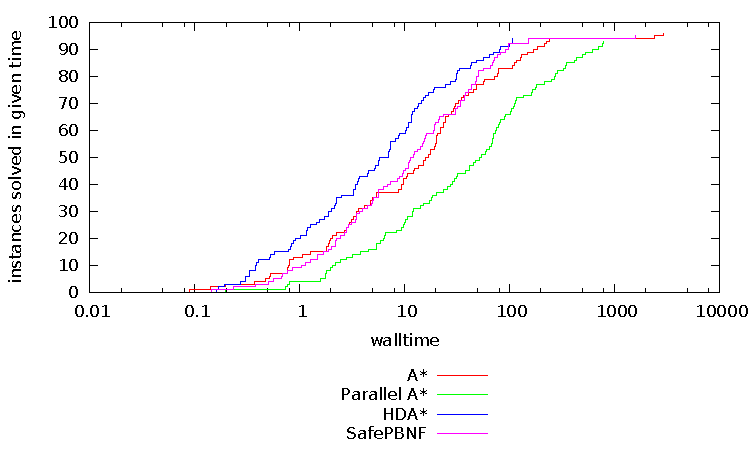
\includegraphics[width=\columnwidth,draft]{eps/15puzzle_vector_walltime.pdf}
		\caption{15 Puzzle (vector)}
		\label{fig:15puzzle_vector}
	\end{subfigure}
	\begin{subfigure}{0.4\columnwidth}
		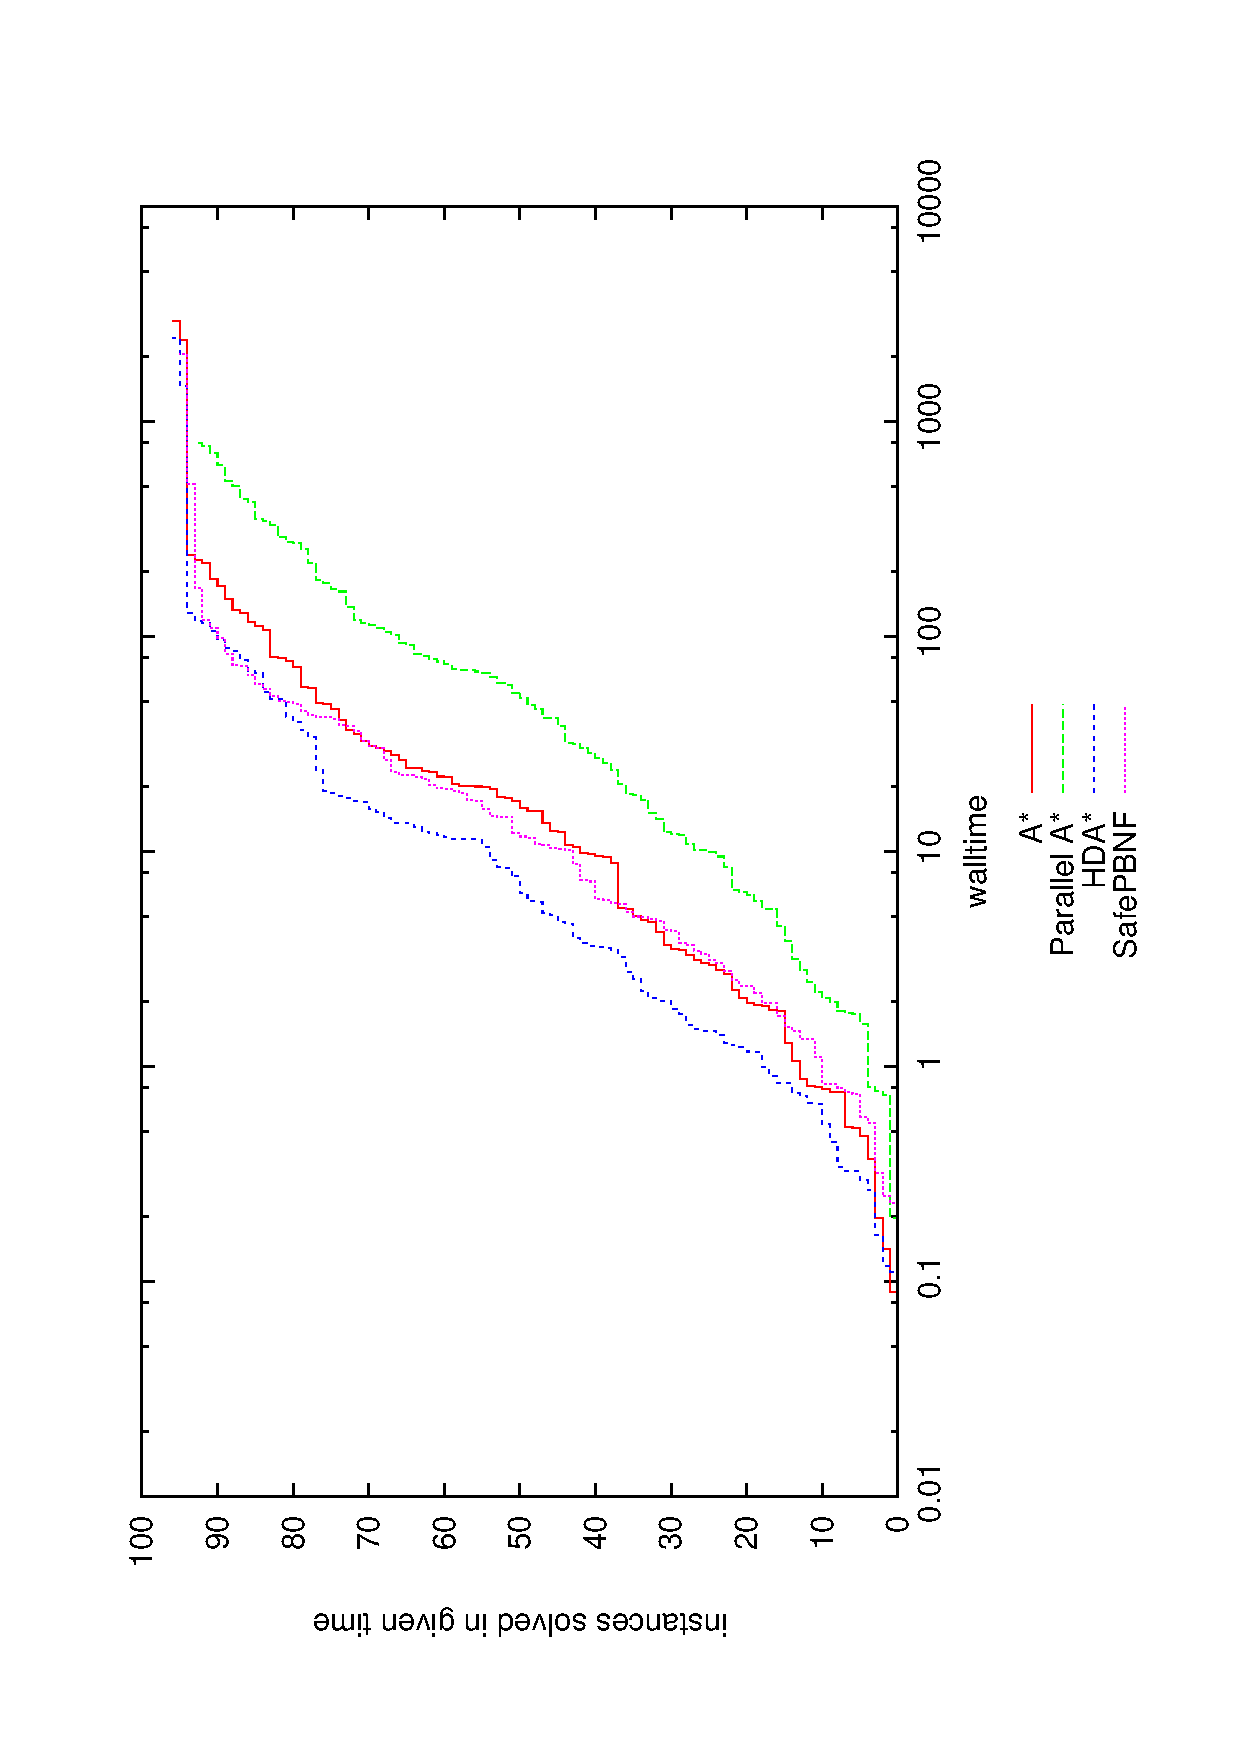
\includegraphics[width=\columnwidth]{eps/15puzzle_heap_walltime.pdf}
		\caption{15 Puzzle (heap)}
		\label{fig:15puzzle_heap}
	\end{subfigure}
	\begin{subfigure}{0.4\columnwidth}
		\includegraphics[width=\columnwidth]{eps/24_walltime.pdf}
		\caption{24 Puzzle (vector)}
		\label{fig:24puzzle_vector}
	\end{subfigure}
	\begin{subfigure}{0.4\columnwidth}
		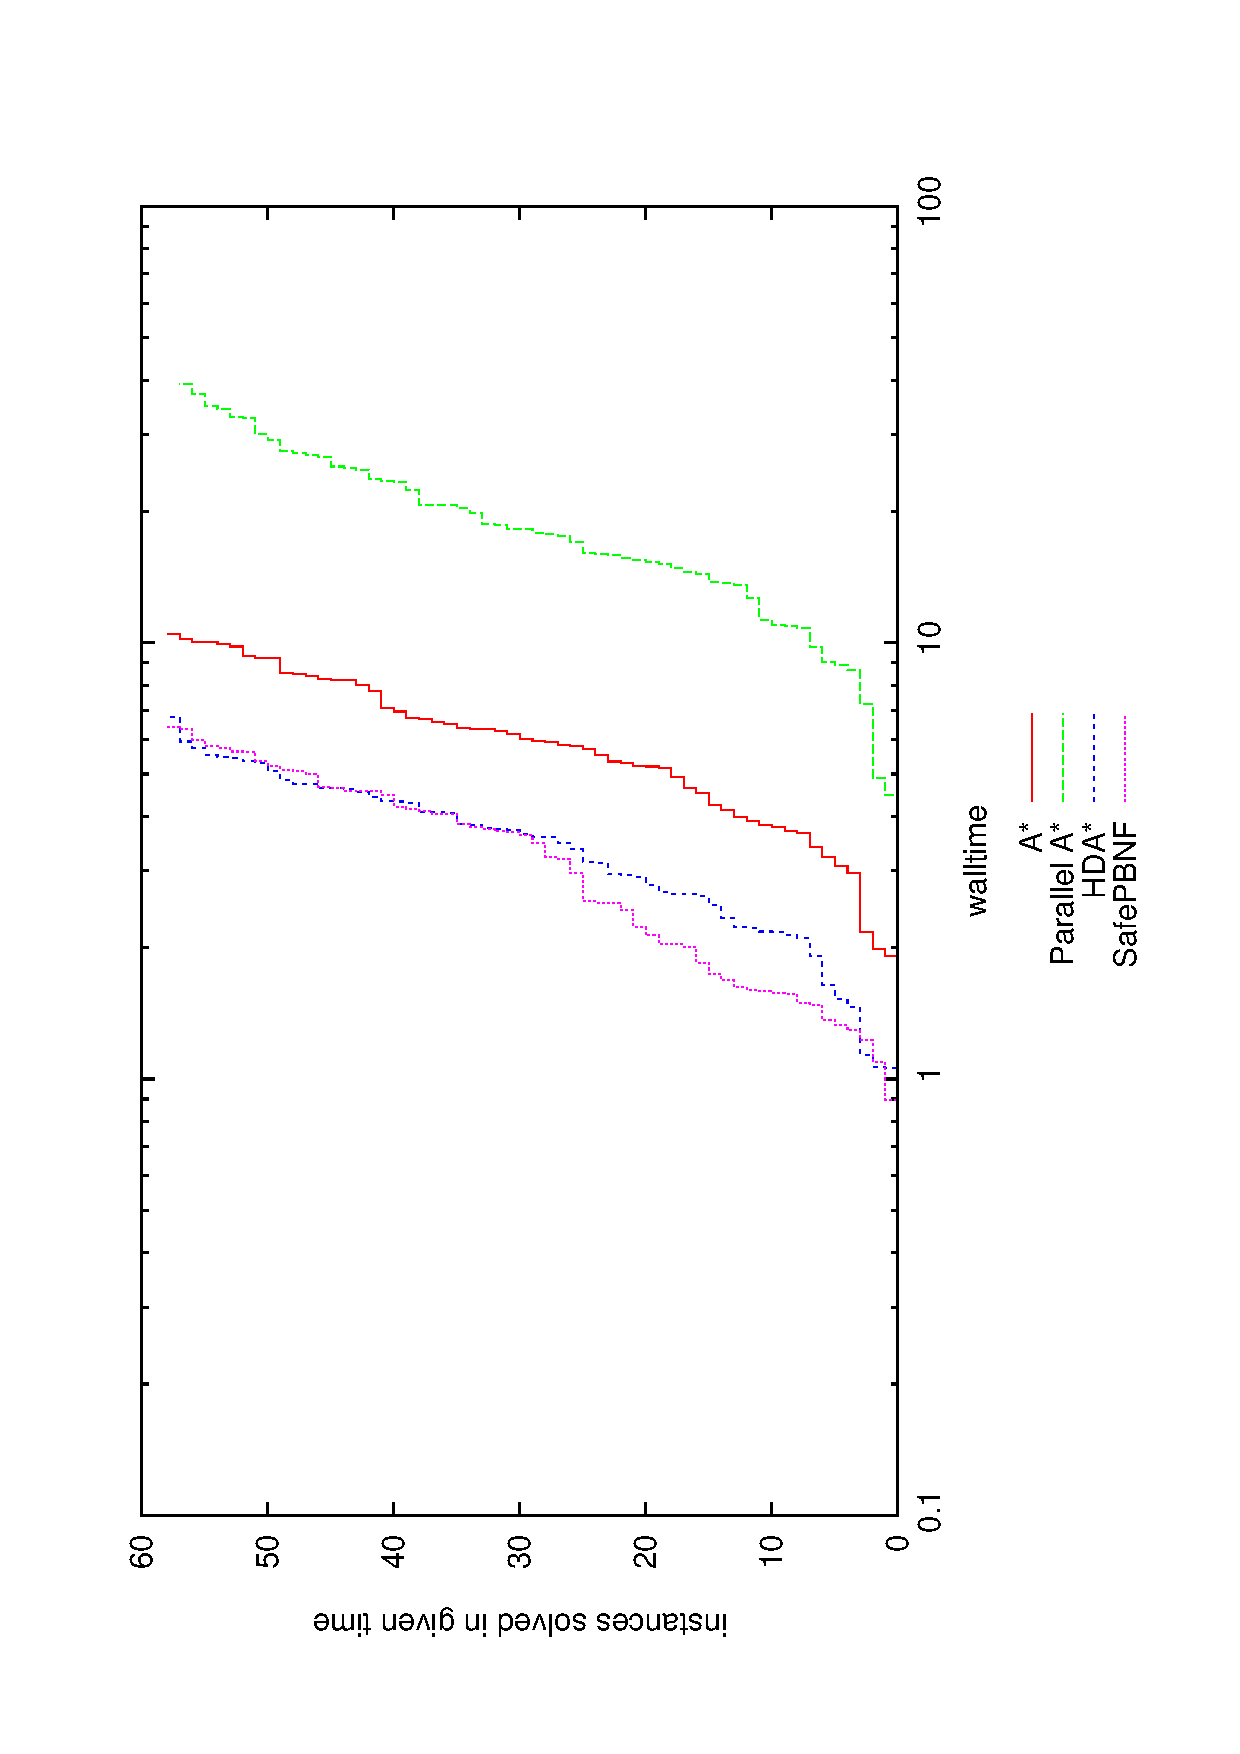
\includegraphics[width=\columnwidth]{eps/grid_walltime.pdf}
		\caption{Grid Pathfinding (vector)}
		\label{fig:grid}
	\end{subfigure}
	\begin{subfigure}{0.4\columnwidth}
		\includegraphics[width=\columnwidth]{eps/tsp_20_walltime.pdf}
		\caption{TSP20 minimum spanning tree (heap)}
		\label{fig:tsp_20_mst}
	\end{subfigure}
	\begin{subfigure}{0.4\columnwidth}
		\includegraphics[width=\columnwidth]{eps/tsp_13_walltime.pdf}
		\caption{TSP13 round trip (heap)}
		\label{fig:tsp_13}
	\end{subfigure}

	\caption{HDA*とSafePBNFの実行速度の比較}
	\label{fig:comparison}
\end{figure}%

\begin{figure}
	\centering
	\begin{subfigure}{0.4\columnwidth}
		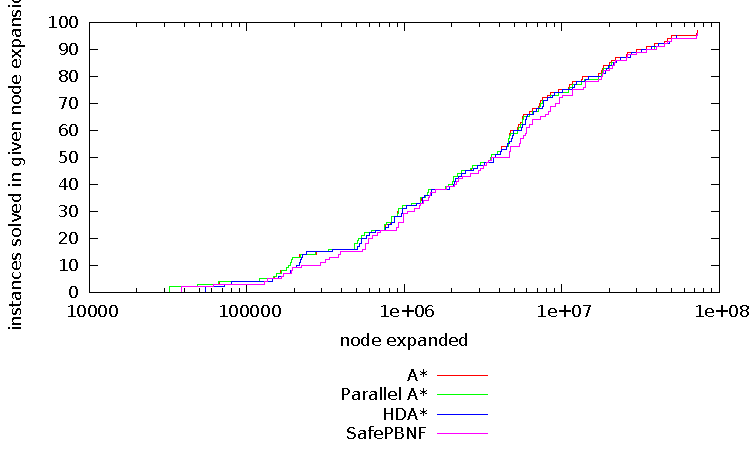
\includegraphics[width=\columnwidth,draft]{eps/15puzzle_vector_expd.pdf}
		\caption{15 Puzzle (vector)}
		\label{fig:15puzzle_vector_expd}
	\end{subfigure}
	\begin{subfigure}{0.4\columnwidth}
		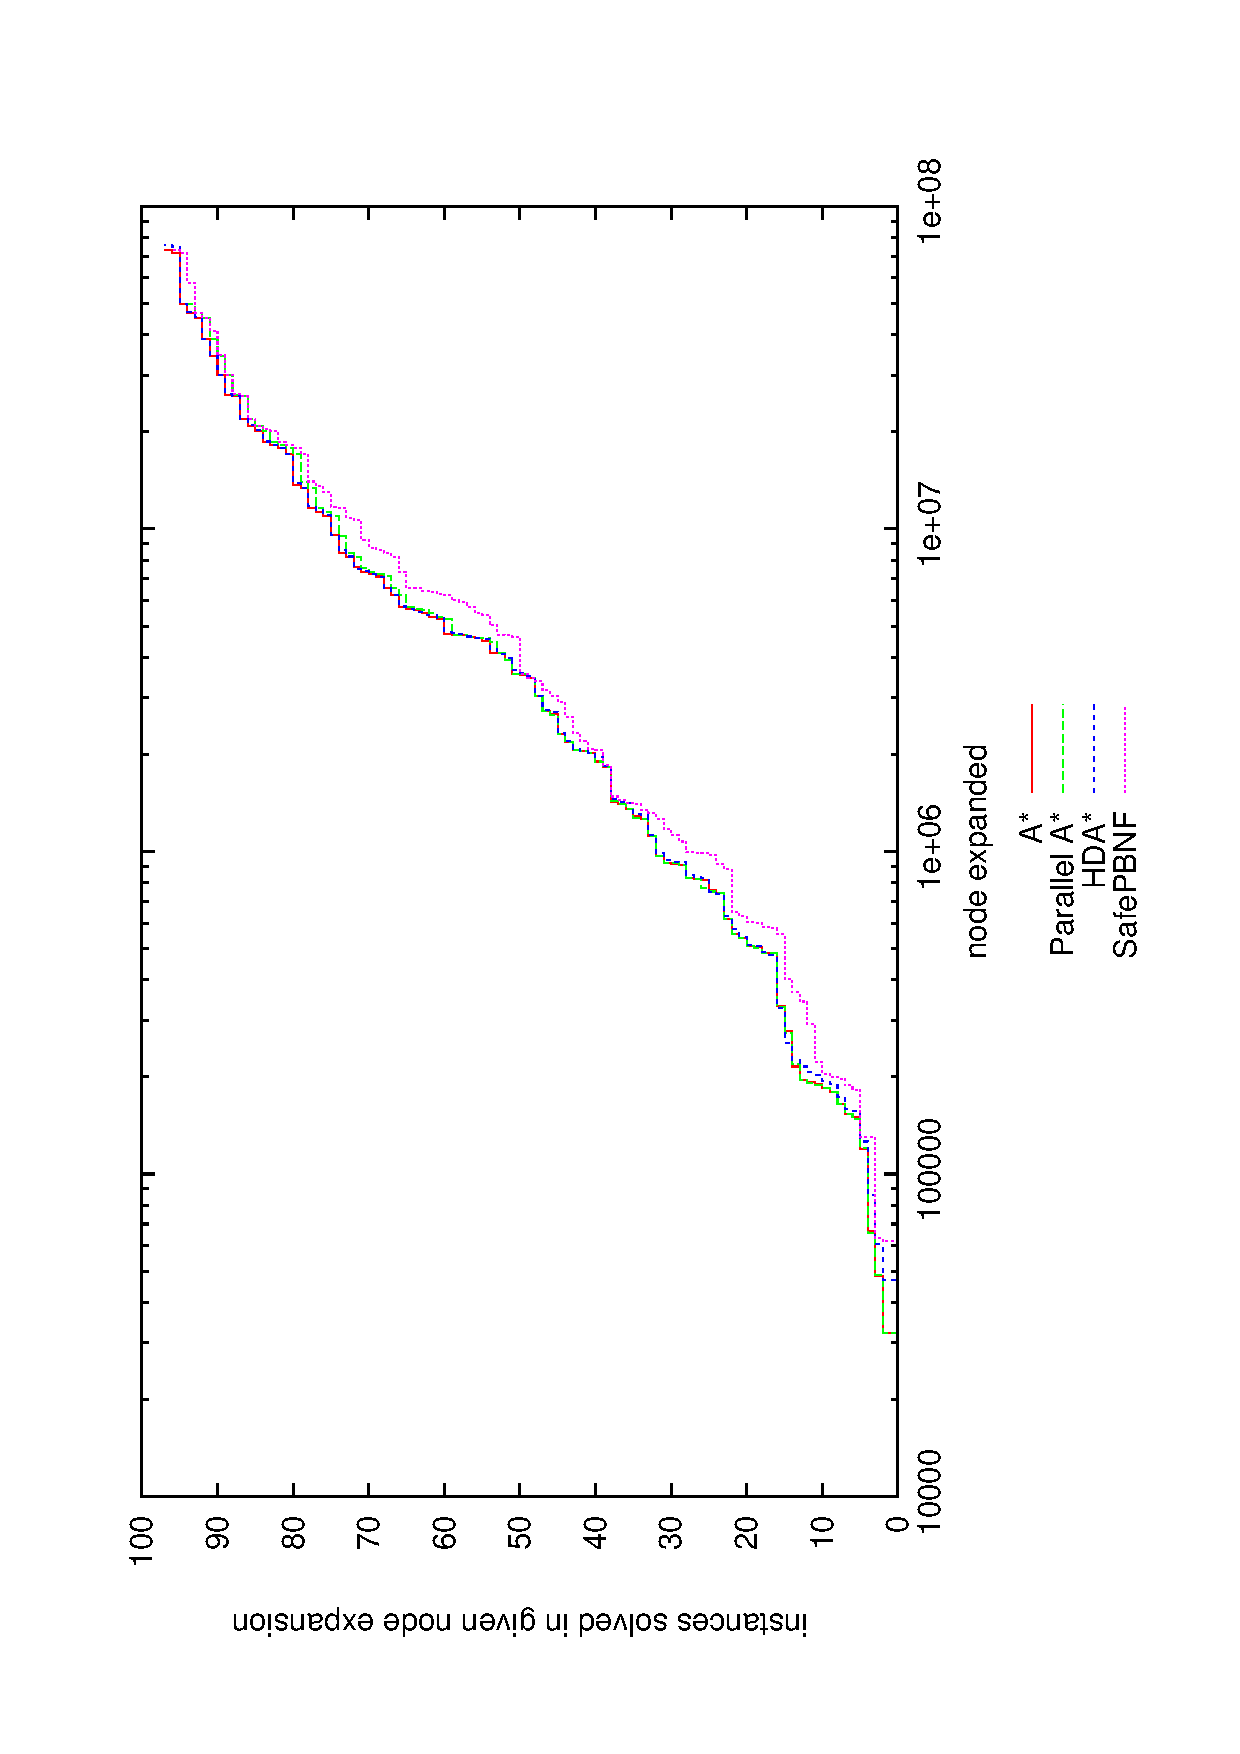
\includegraphics[width=\columnwidth]{eps/15puzzle_heap_expd.pdf}
		\caption{15 Puzzle (heap)}
		\label{fig:15puzzle_heap_expd}
	\end{subfigure}
	\begin{subfigure}{0.4\columnwidth}
		\includegraphics[width=\columnwidth]{eps/24_expd.pdf}
		\caption{24 Puzzle (vector)}
		\label{fig:24puzzle_vector_expd}
	\end{subfigure}
	\begin{subfigure}{0.4\columnwidth}
		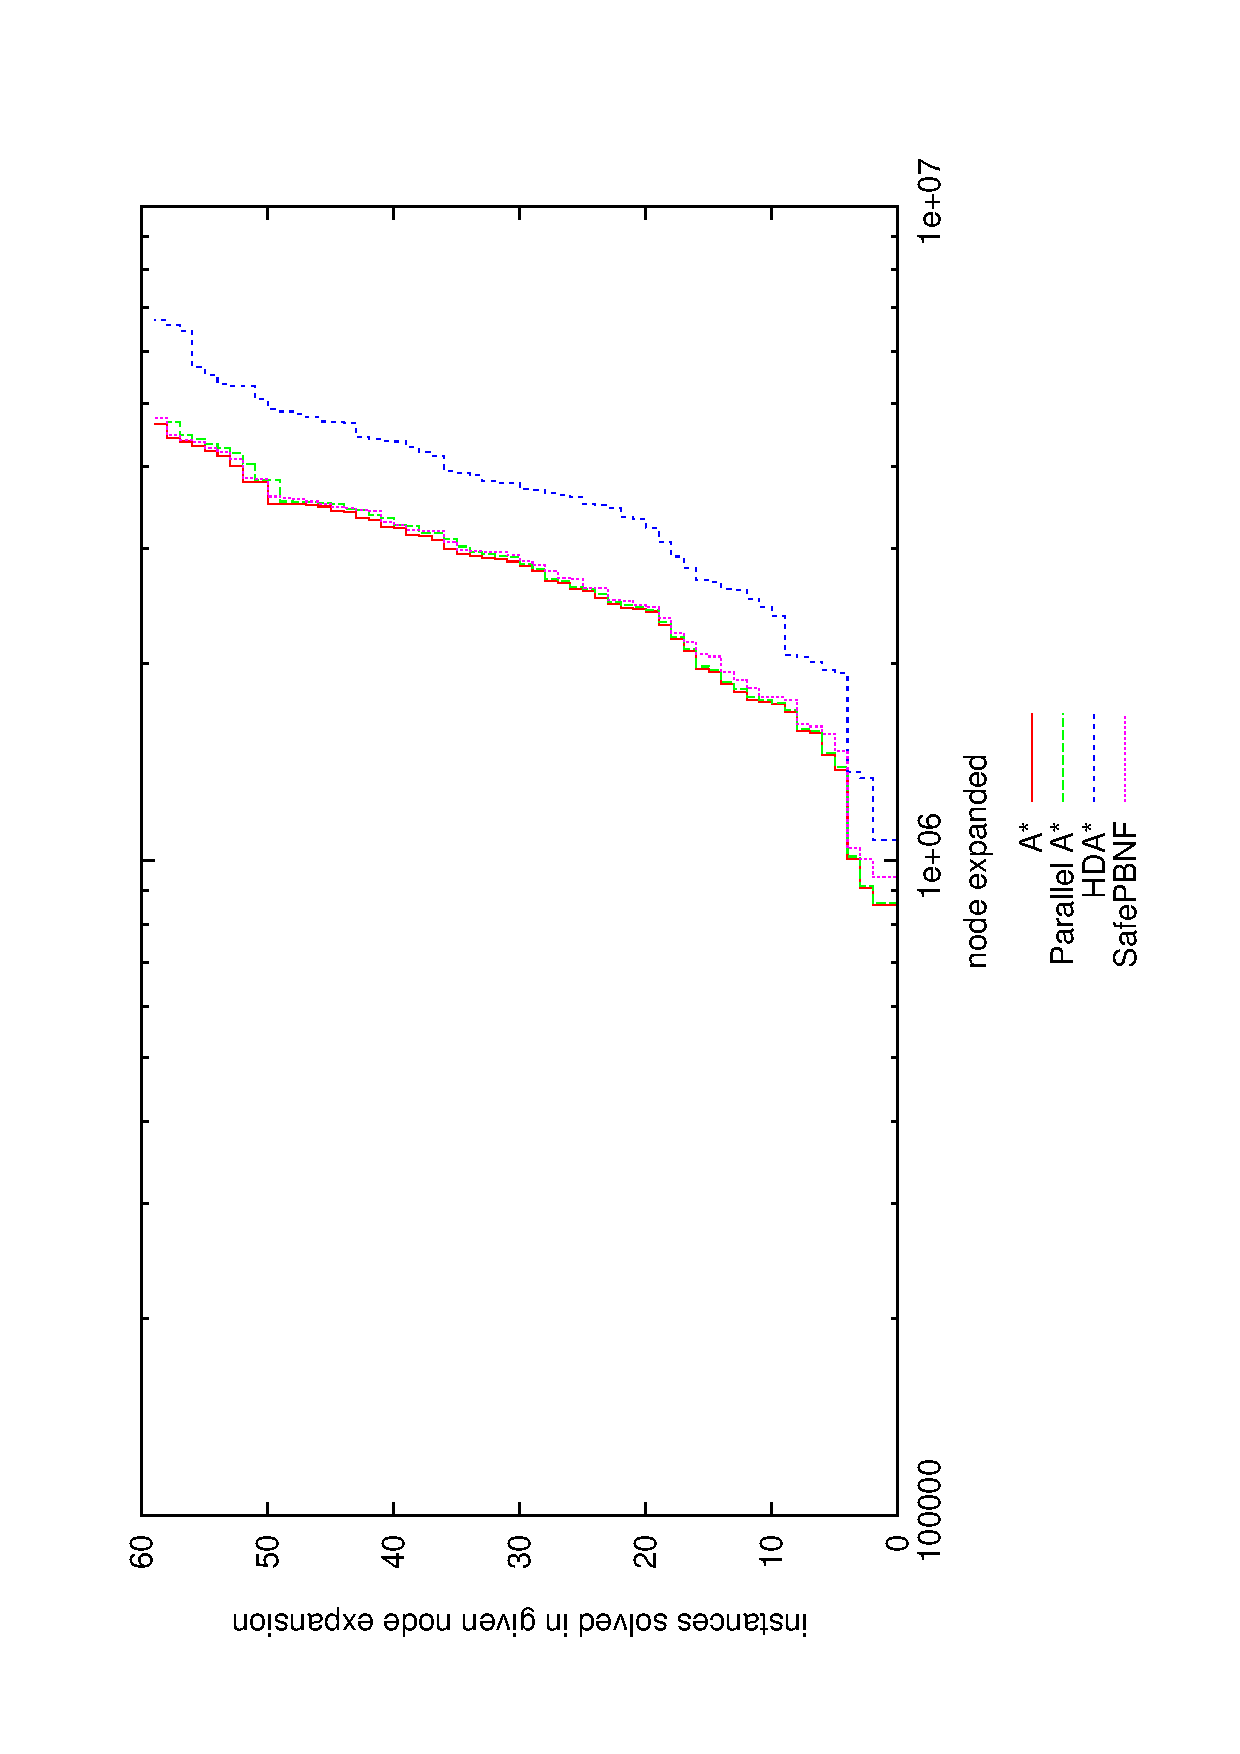
\includegraphics[width=\columnwidth]{eps/grid_expd.pdf}
		\caption{Grid Pathfinding (vector)}
		\label{fig:grid_expd}
	\end{subfigure}
	\begin{subfigure}{0.4\columnwidth}
		\includegraphics[width=\columnwidth]{eps/tsp_20_expd.pdf}
		\caption{TSP20 minimum spanning tree (heap)}
		\label{fig:tsp_20_mst_expd}
	\end{subfigure}
	\begin{subfigure}{0.4\columnwidth}
		\includegraphics[width=\columnwidth]{eps/tsp_13_expd.pdf}
		\caption{TSP13 round trip distance (heap)}
		\label{fig:tsp_13_expd}
	\end{subfigure}
	\caption{HDA*とSafePBNFの展開ノード数の比較}
	\label{fig:comparison_expd}
\end{figure}%


図\ref{fig:comparison}が実行速度の比較である。それぞれの図は、横軸に実行時間、縦軸にその実行時間内に解ける問題の数を示してある。これらの結果から、特に実行時間の大きい問題ドメイン・インスタンスにおいて、HDA*はSafePBNFよりもパフォーマンスに優れると結論出来る。一方、実行時間が5秒未満程度の小さい問題に対してはSafePBNFの方が優れる場合が多い。\ref{sec:analysis1}章で述べたように、HDA*は実行時間の冒頭と末尾に探索オーバーヘッドがある。実行時間が短い場合、これらのオーバーヘッドの割合が大きくなる。よって、小さな問題インスタンスに対しては探索オーバーヘッドが大きく、SafePBNFの方が速いと考えられる。特にGrid Pathfindingの1秒程度の問題においてHDA*は大きな探索オーバーヘッドを持つ。
\newline

図\ref{fig:comparison_expd}は展開ノード数の比較である。それぞれの図は、横軸に展開ノード数、縦軸にその展開ノード数以内に解ける問題の数を示してある。実行時間の短いGrid Pathfindingを除き、HDA* vs. SafePBNFの展開ノード数はあまり変わらない。\ref{sec:analysis1}章の結論とこの結果を踏まえると、HDA*は十分に大きな問題に対しては探索オーバーヘッドの殆どない手法であると結論出来るだろう。BurnsらがHDA*の探索オーバーヘッドを指摘したのはHash関数をNaive Hashで実装したからである。図\ref{fig:order_naive_hash}及び図\ref{fig:hdastar_tuning}より、Naive Hashは明らかに不均一なHash関数である。
\newline

図\ref{fig:15puzzle_heap}は15 Puzzleに対してheapで実装した場合の実行時間である。SafePBNFの利点として、Burnsらはオープンリストが小さい為、heapへのアクセスが速いということと挙げた\cite{Burns2010}。しかし、この実験結果はheap実装においてもHDA*がSafePBNFよりもパフォーマンスに優れるということを示す。
\newline

シンプルなParallel A*は逐次A*よりも遅くなってしまう。Parallel A*はオープンリストとクローズドリストにロックを必要とする。スレッドはロックが解放されるのを待たなければならない為、大きな同期オーバーヘッドが生じる。この結果はBurnsらの実験と一致する\cite{Burns2010}。
\newline

\begin{table}
	\centering
	\begin{tabular}{lrrrr} \hline
		 & &             HDA* & & SafePBNF \\ 
		 &  解の発見回数 & 最初の解の発見時間 & 解の発見回数 & 最初の解の発見時間 \\ \hline
		15 Puzzle & 1 & 14.56 & 1.14 & 20.73 \\ 
		24 Puzzle & 1 & 59.82 & 1 & 67.04 \\ 
		Grid Pathfinding & 1.02 & 3.45 & 1.02 & 3.30 \\ 
		TSP20 (MST) & 1 & 5.18 & \textbf{2.25} & \textbf{1.23} \\ 
		TSP13 (RTD) & 1 & 16.80 & \textbf{2.60} & \textbf{8.56} \\ \hline
	\end{tabular}
	\caption{解の発見回数と最初の解の発見時間の平均}
	\label{hdastar_incumbent}
\end{table}

% TSPはSafePBNFが得意な問題ドメインであると考えられる。空間を簡単に分割することが出来る為である。
表\ref{hdastar_incumbent}はHDA*とSafePBNFにおいて、解を発見した平均の回数である。SafePBNFの探索方法はAnytime Searchのような特徴を持つ\cite{Burns2010}。すなわち、SafePBNFは最適でない解を素早く見つけ、時間と共により良い解を発見することが出来る。最適でない解を発見した場合、その解のコストよりもコストの大きいノードを生成する必要がなくなる。ノードの生成は探索時間の大きな割合を占める為、生成の回数を減らすことは大きな高速化につながる。TSPは深さが都市の数と同じノードは全て解である。都市が20個の場合は$20!/2$通りの解が存在する。SafePBNFは解が無数にあるTSPでは素早く解を発見でき、その為最適解も高速に見つけられると考えられる。


\section{おわりに}
\label{sec:conclusion}

本研究の貢献は大きく分けて2つある。

\begin{enumerate}
\item HDA*の探索オーバーヘッドの定性的な分析

HDA*の探索オーバーヘッドの原因を3つに分類を行い、十分問題サイズが大きい場合に探索オーバーヘッドが無視出来る程度に小さいことを理論的に示した。また、高速化効率と探索オーバーヘッドを問題インスタンス毎に示すことで、それを実験的にも証明した。本実験は共有メモリ環境において行われたが、分散メモリ環境においても同様の結果が得られると推測している。その実験的な実証は今後の研究課題である。また、本研究は新しい探索オーバーヘッドの分析手法を示した。これは他の並列探索においても有効な分析方法であると考えられる。
\newline

\item HDA*とPBNFの再評価

先行研究の分析の問題点を指摘し、より正確かつミクロな分析を行った。実験により、マルチコア環境においても相応しい実装を行えばHDA*の方がパフォーマンスに優れるという結果を得た。また、本研究ではOptimal Searchを対象としたがSuboptimal Searchにおける実験は行っていない。Suboptimal Searchにおける性能比較は今後研究課題である。簡易ヒューリスティックを用いたTravelling Salesperson ProblemにおいてはSafePBNFの方がHDA*よりも速いという結果を得た。これはSafePBNFのheapの方が小さい為、heapへのアクセスが速い為ではないかと考えられる。heapは複数に分割することが出来る。分割heapを用いることで実数コストドメインにおけるHDA*, SafePBNFのパフォーマンスを向上させることが出来るかもしれない。これは今後の研究課題である。

\end{enumerate}

\section{謝辞}

研究室の先輩方にはミーティングや中間発表などで沢山の有益なアドバイスを頂きました。特に同期の堀江君とは本当に毎日議論を重ね、沢山のことを学ばせて頂きました。指導教員である福永先生には、初めて情報科学に触る私に対してとても丁寧にご指導して頂きました。研究とは、情報科学とは、プログラミングとは、あらゆることを教えて頂きました。何よりも、研究が楽しいということを教えて頂いたことに深く感謝致します。修士課程でも、一つでも多くのことを学ばせて頂きたいと思います。

\newpage

\bibliographystyle{jplain}
\bibliography{b}

\newpage

\printindex

\end{document}
